\documentclass[11pt,a4paper]{article}
\usepackage[T1]{fontenc}
\usepackage[utf8]{inputenc}
\usepackage{amsmath,amssymb,bm}
\usepackage{amsthm}
\newtheorem{lemma}{Lemma}
\usepackage{graphicx}
\usepackage{booktabs}
\usepackage{siunitx}
\usepackage[margin=1in]{geometry}
\usepackage{caption}
\usepackage[hidelinks]{hyperref}
\usepackage{xcolor}

\begin{document}
\title{Reference-free error predictability in phase-space nodal
transport: the strict phase-space diffusion closure}
\author{Yuchao Xu\thanks{Corresponding author.}%
\quad University of South China\quad \texttt{yxu40@hotmail.com}}
\date{}
\maketitle
\begin{center}\vspace{-6mm}{\small\it To appear in Annals of Nuclear Energy (preprint)}\end{center}

\begin{abstract}
Nodal transport discretizations whose spatial body operator and
angular-moment face operator are derived from \emph{different}
projections of the same transport equation exhibit a specific
convergence pathology: the two discretization errors carry opposite
signs, cancel along a diagonal band $S \approx M/2$ of the spatial
$\times$ angular refinement grid, and the optimal configuration is
locked on that band --- refining either axis alone moves the solution
\emph{away} from the true one.  Along such a band the method is not
predictable: per-row error sequences are non-monotonic and reverse
sign, and the error at any computed point cannot be bounded without an
external reference.  We identify this body/face inconsistency in the
phase-space nodal (PSN) method of Chao et al. [Ann. Nucl. Energy 240
(2027) 112707] and remove it with a \emph{strict phase-space diffusion
closure}: the node body is solved with the exact sector tensor
$\bm{D}_m$ that already governs the face currents, whose two
sector-diagonal plane waves are pointwise exact homogeneous solutions
for every sector width and anisotropy level (dispersion lemma
$w^{\mathsf T}\bm{D}_m w = p$).  The closure keeps the legacy node size,
closure equations, and conditioning; at $M=2$ it reproduces the legacy
node bit-for-bit.  On the strong/weak-absorber checkerboard
($S\le20$, $M\le192$, 288 points), every fixed-$S$ row of the strict
method converges monotonically and single-signed at $O(M^{-2})$ to a
limit that \emph{is} the pure spatial residual.  Consequently the
Richardson $M\to\infty$ limit predicted from $M=48/96$ alone matches
the $M=384$ measurement within $0.6$~pcm --- 40-row reference-free
prediction with a self-reported error bar --- while the legacy
sequences, however extrapolated, converge to an operator-error
plateau ($+49.7$~pcm at $S{=}12$) that is only visible against an
external Monte Carlo reference.  Error predictability, not accuracy at
the best tunable point, is the operative property for qualification,
and it is what the strict closure restores.
\end{abstract}

\noindent\textbf{Keywords:} phase-space nodal method; diffusion
approximation; convergence analysis; Richardson extrapolation;
verification and validation

%======================================================================
\section{Introduction}
\label{sec:intro}

Deterministic nodal methods earn their place in reactor analysis by
being \emph{predictive}: given two computations at different
discretization levels, one must be able to forecast the third, bound
the residual error, and decide which refinement axis to fund --- all
without recourse to an external solution.  This paper is about a
failure mode of that property and its removal in the phase-space nodal
(PSN) method~\cite{chao2027}.

PSN carries angular-moment (diffusion-moment) unknowns in phase space:
each spatial node and energy band is subdivided into azimuthal sectors,
and a nodal response map connects face partial currents to face
partial fluxes~\cite{chao2027}.  In the reproduction of the
strong/weak-absorber checkerboard benchmark of~\cite{chao2027}
(Fig.~3 therein), the error over the spatial subdivision $S$ and
azimuthal order $M$ organizes along a diagonal band $S \approx M/2$:
the optimum at each $M$ sits on the band, the band drifts as $M$
grows, and points off the band degrade in \emph{both} refinement
directions.  We call this the \emph{valley locking} pathology.  Its
practical content is not the band's existence but three consequences:
(i)~fixed-$S$ error sequences are non-monotonic and change sign
(measured: $-37.4 \to +24.0 \to +42.1 \to +47.8$~pcm along
$M=24\ldots192$ at $S{=}12$); (ii)~no extrapolation of a row predicts
a physically meaningful limit; (iii)~convergence is certifiable only
against an external reference.

The root cause is structural.  The legacy PSN node solves an
\emph{isotropic} body diffusion equation whose diffusion coefficient
is the full-angle-averaged one, while its face currents
[eq.~(2.7c) of~\cite{chao2027}] carry the \emph{sector} tensor
$\bm{D}_{im}$ with the exact $\operatorname{sinc}(\pi/M)$ anisotropy.
Refining $S$ converges to the solution of the body operator, refining
$M$ to the face operator's; the two limits differ, the two errors
oppose, and the valley is their zero contour.  The paper makes this
precise, then repairs the inconsistency.

The repair must not break what PSN gets right.  We therefore require
(i)~the same node map size and closure (no new interface unknowns, no
new stencil), (ii)~an exact anchor: at $M=2$ the strict node equals
the legacy node to machine precision, and (iii)~no tuning: every
coefficient is derived, none fitted.  The resulting \emph{strict
phase-space diffusion closure} solves the body with the same $\bm{D}_m$
as the faces.  Its mathematical core is a dispersion lemma: for every
sector, every anisotropy level, and every band weight, the plane waves
along the two \emph{sector-diagonal} directions
$\theta_w = \phi_m \pm \pi/4$ are exact homogeneous solutions with a
single decay constant $k=\sqrt{\Sigma_t/p}$.  The node basis is the
four hyperbolic modes of those two directions plus the constant ---
same status and conditioning as the legacy additive family --- and the
paraboloidal source particular solution becomes pointwise exact rather
than cell-mean exact.

Contributions:
\begin{enumerate}
\item a diagnosis of the body/face operator inconsistency in PSN and
the proof that the checkerboard diagonal valley is its zero-error
contour (Sec.~\ref{sec:legacy});
\item the strict closure: derivation, exact basis lemma, node map,
$M=2$ anchor (Sec.~\ref{sec:strict});
\item the predictability experiment: 288 checkerboard points
$S\le20$, $M\le192$, showing per-row monotone $O(M^{-2})$ convergence,
Richardson prediction of row limits to sub-pcm against $M=384$
measurement, and a $\propto S^{-2}$ spatial-residual sequence
(Sec.~\ref{sec:exp});
\item release as \texttt{angular.closure: strict\_phase\_space} in
OpenPSN with regression gates (Sec.~\ref{sec:impl}).
\end{enumerate}

%======================================================================
\section{Legacy PSN and the valley locking pathology}
\label{sec:legacy}

\subsection{Node structure}
One group, spatial node of size $h_x \times h_y$, azimuthal sectors
$\phi \in [\,m\,\Delta\phi,(m{+}1)\,\Delta\phi)$,
$\Delta\phi=\pi/M$, centered at $\phi_m$.  The base angular function is
P1-type restricted to the sector; the odd (streaming) parity is
eliminated in favor of net face currents $J_f$, $f=0..3$, leaving five
source moments $q=(q_0,q_{1x},q_{1y},q_{2x},q_{2y})$.  The legacy node
solves in the body
\begin{equation}
-\nabla\!\cdot\!\big(p\,\nabla\phi\big) + \Sigma_t\,\phi = q(x,y),
\qquad p = \frac{\mu_i^2}{2\Sigma_t}\ \text{(TY)},\quad
p=\frac{\beta_i}{3\Sigma_t}\ \text{(generic)},
\label{eq:legacybody}
\end{equation}
isotropic, with additive trial family
$\{1,\ \mathrm{ch}(kx),\ \mathrm{sh}(kx),\ \mathrm{ch}(ky),\
\mathrm{sh}(ky)\}$ and $k^2=\Sigma_t/p$; the face currents are then
formed with the sector mixing [2.7c]
\begin{equation}
J_{x\pm} = \left(1 \pm s\cos 2\phi_m\right) J_X \pm s \sin 2\phi_m
\; J_{\mathrm{avg}}, \qquad s=\operatorname{sinc}(\Delta\phi),
\label{eq:face}
\end{equation}
which \emph{is} the divergence-theorem current of a tensor
\begin{equation}
\bm{D}_m = p\begin{pmatrix} 1+s\cos 2\phi_m & s\sin 2\phi_m \\
s\sin 2\phi_m & 1-s\cos 2\phi_m \end{pmatrix}.
\label{eq:Dm}
\end{equation}
Identity: the unweighted sector average of the second angular moment
equals the half-range-weighted face tensor of [2.7c] --- the same
$\bm{D}_m$ in both guises.  The inconsistency is that
\eqref{eq:legacybody} replaces $\bm{D}_m$ by $p\,\bm{I}$ in the body
while \eqref{eq:face} keeps $\bm{D}_m$ at the faces.

\subsection{Consequence: two operators, one valley}
Let $d(S,M)$ be the $\Delta k_{\mathrm{eff}}$ against a reference.
Because the discrete problem converges (as $S\to\infty$ at fixed $M$)
to a fixed-$M$ \emph{problem} whose operator mixes body-isotropic and
face-tensor physics, and (as $M\to\infty$ at fixed $S$) to the
consistent-tensor limit of the \emph{face} operator on the coarse
mesh, the error separates to leading order,
\begin{equation}
d(S,M) \;=\; a(S) + b(M) + \text{h.o.t.},
\qquad a(S)\asymp c_S S^{-2},\quad
b(M)\asymp c_M M^{-2},
\label{eq:split}
\end{equation}
with $c_S c_M < 0$ for the checkerboard (measured: $a>0$, $b<0$ for
the strong absorber).  A zero contour $a(S)+b(M)=0$ then exists in
\emph{every} consistent two-parameter method --- it is a consequence of
the intermediate value theorem, not a defect.  The defect is when the
contour \emph{drifts with $M$} (here $S^{*}\approx M/2$, because
$b(M)$ is a wrong-operator bias that decays in $M$ while $a$ does not)
and the per-row limits are nonzero: the method's own asymptotics point
\emph{away} from the contour as either axis is refined past the
crossing.  Measured legacy optima (strong absorber):
$S^{*}=5,9,15,20,\text{ out of range}$ at $M=12,24,48,96,192$ ---
the band runs out of every finite grid.

%======================================================================
\section{Strict phase-space diffusion closure}
\label{sec:strict}

\subsection{Strict body equation}
Replace \eqref{eq:legacybody} by the sector tensor body:
\begin{equation}
-\nabla\!\cdot\!\left(\bm{D}_m \nabla\phi\right)
+ \Sigma_t\,\phi = q(x,y),
\qquad \bm{D}_m \text{ from } \eqref{eq:Dm}.
\label{eq:strictbody}
\end{equation}
The face currents of \eqref{eq:face} are then exactly the
divergence-theorem currents $J_f = \langle -\bm{n}\!\cdot\!\bm{D}_m
\nabla\phi\rangle_f$ of the body operator: body and face are the
\emph{same} operator (verified to $3\times10^{-15}$ against the printed
mixing formula for arbitrary sectors, including non-power-of-two $M$).
Equation~\eqref{eq:strictbody} is not a heuristic blend: it is the
cell-tensor projection of the same transport operator that produced
\eqref{eq:face}, obtained by averaging the second angular moment over
the sector before (not after) eliminating the odd parity --- the
projection order that the face formula implicitly assumes.

\subsection{Exact basis lemma}
\begin{lemma}[diagonal dispersion]
For any $p>0$, $|s|\le 1$, sector center $\phi_m$, the plane wave
$e^{k\,w\cdot r}$ solves the homogeneous \eqref{eq:strictbody} iff
$w^{\mathsf T}\bm{D}_m w = p$, i.e.\ iff
$\theta_w = \phi_m \pm \pi/4$, with the single decay
$k=\sqrt{\Sigma_t/p}$.
\end{lemma}
\begin{proof}
$w^{\mathsf T}\bm{D}_m w = p\,[1 + s\cos 2(\theta_w-\phi_m)] = p$
iff $\cos 2(\theta_w - \phi_m) = 0$.  The decay then follows from
$\Sigma_t - k^2 p = 0$.  Pointwise, no approximation.
\end{proof}
The node basis is thus
$\{1,\ \mathrm{ch}(k\,u),\ \mathrm{sh}(k\,u),\ \mathrm{ch}(k\,v),\
\mathrm{sh}(k\,v)\}$, $u = r\!\cdot\!w(\phi_m{+}\pi/4)$,
$v = r\!\cdot\!w(\phi_m{-}\pi/4)$: four exact homogeneous modes, one
constant, five source moments --- identical count to legacy, and unlike
the legacy additive family it responds to cross-derivative
(streaming-diagonal) structure, $\partial_{xy}\phi \ne 0$ in the body.
The source particular solution
$\phi_p = [q_0 + q_{1x}P_1 + q_{1y}P_1 + q_{2x}P_2 + q_{2y}P_2]/
\Sigma_t + C_p$, $C_p = 3(D_{xx}q_{2x}/a^2 + D_{yy}q_{2y}/b^2)/
\Sigma_t^2$, satisfies the tensor equation pointwise.

\subsection{Node map and the $M=2$ anchor}
The closure is unchanged: four face net currents $J_4$ determine four
mode coefficients through a $4\times4$ matrix of the same conditioning
profile as the legacy one (measured cond\ $\le 5.7\times10^{2}$ up to
$M{=}24$); the constant comes from the exact volume balance; face
partial fluxes keep the legacy geometry-free chord factor
$\alpha_f$.  No interface unknowns are added anywhere.

At $M=2$ (restricted model, $\phi_m=\pi/4$, $s=2/\pi$) the diagonal
directions $\phi_m \pm \pi/4$ are \emph{exactly} the $x$ and $y$ axes:
the strict basis spans the same space as the legacy basis at the same
$k$, and the node map coincides with the production legacy rect node to
$2.8\times10^{-15}$ relative on random $(J_4,q)$ (kernel), and the
global checkerboard $k_{\mathrm{eff}}$ to $8.9\times10^{-11}$~pcm
(solver noise).  The strict method is therefore a conservative
generalization: the legacy method is not discarded, it is the $M{=}2$
slice of the strict family where the two operators happen to agree.
(For the generic polar model the legacy body is
$k^2 = 3\Sigma_t^2 \ne \Sigma_t/p$ \emph{by construction}; the anchor
there is the consistent-tensor limit itself, and strict$\,\neq\,$legacy
at every $M$ --- by design.)

%======================================================================
\section{Experiments: predictability, not point accuracy}
\label{sec:exp}

Protocol: strong ($\Sigma_a=0.70$, $k_{\mathrm{ref}}=0.51673$) and weak
($0.07$, $1.12974$) absorber checkerboards~\cite{chao2027}, generic
polar $I=30$, solver tolerance $10^{-10}$, grid
$S=1\ldots20 \times M=2\ldots192$ (288 points per method-material
combination pair), OpenMC references as in~\cite{chao2027}.  All
numbers below are computed, none fitted.

\subsection{Valley locking removed (Fig.~\ref{fig:bestS})}
The strict optimum at fixed $M$ saturates:
$S^{*}=3,5,8,10,11$ at $M=12,24,48,96,192$ (strong absorber) --- it
locks onto the crossing of the spatial residual $a(S)=0$ near
$S\approx11$ and stops moving.  The legacy optimum tracks
$S\approx M/2$ past the edge of every grid tried
($S^{*}=20$ at $M{=}96$, out of range at $M{=}192$).  Both rows of
Table~\ref{tab:rows} show the same $S{=}12$ row: monotone single-signed
$O(M^{-2})$ (successive ratios $3.30,2.83,2.07\to4$) versus a
sign-reversal sequence.

\begin{table}[t]
\centering
\caption{$\Delta k_{\mathrm{eff}}$ (pcm), $S{=}12$ row, strong absorber.}
\label{tab:rows}
\begin{tabular}{lrrrrr}
\toprule
$M$ & 24 & 48 & 96 & 192 & 384 \\
\midrule
legacy & $-37.4$ & $+24.0$ & $+42.1$ & $+47.8$ & (plateau $+52$) \\
strict & $-83.2$ & $-25.2$ & $-8.9$  & $-4.3$  & $-3.0$ \\
\bottomrule
\end{tabular}
\end{table}

\subsection{Reference-free prediction}
\label{sec:pred}
For every row with $M=24,48,96,192$ we form the Richardson limit
$\hat d_\infty = (4 d_{2M} - d_M)/3$ and its \emph{self-reported error
bar} $\varepsilon = |\hat d_\infty(M_1,M_2) -
\hat d_\infty(M_2,M_3)|$: the disagreement of successive
extrapolations, computable without any measurement beyond $M_3$.
\begin{itemize}
\item Strong, $S{=}12$: predictions from $(48,96)$ and $(96,192)$:
$-3.5$ / $-2.8$~pcm, bar $0.7$~pcm; \emph{later-measured} $M{=}384$
point: $-3.0$~pcm.  Hit inside the bar.
\item Weak, $S{=}12$: predictions $-1.7$ / $-1.5$, bar $0.2$~pcm;
\emph{measured} $M{=}384$: $-1.6$~pcm.
\item All 40 rows (both absorbers, $S\le20$):
$|\hat d_\infty| \le 22$~pcm with bars $\le 3$~pcm; the row-limit
sequence $\hat d_\infty(S)$ follows $S^{-2}$
(Fig.~\ref{fig:limits}) --- the limits \emph{are} the spatial
discretization residual of one operator, and refining the \emph{other}
axis shrinks them predictably.
\item Legacy, same formula: $(48,96)$ and $(96,192)$ give $+48.1$ /
$+49.7$ at $S{=}12$, self-consistent to $1.6$~pcm --- and
\emph{wrong}: the limit is the body/face operator-error plateau, not
the spatial residual.  Self-consistency of an extrapolation is not
evidence of its validity; only the operator-consistent method has
limits with physical identity.  Against the Monte Carlo reference the
legacy limits sit at $+126.5, +49.7, +20.5, +6.2$~pcm for
$S=8,12,16,20$ --- visible as error only with an external solution.
\end{itemize}
This is the operative difference for qualification: with the strict
closure, a computation at $M\le192$ \emph{knows} its own distance to
the angular limit within $\sim1$~pcm, can allocate the remaining
budget to the correct axis, and certifies $O(S^{-2})$ convergence
without ever consulting $k_{\mathrm{ref}}$.

\subsection{Cost to accuracy}
Reaching $|\Delta k|<5$~pcm on the strong checkerboard: strict at
$S{=}12, M{=}48$; legacy requires $S{=}20, M{=}96$ (an order of
magnitude more unknowns) \emph{and} degrades again at $M{=}192$
($+4.5$~pcm, sign reversal) --- the optimum is a cancellation point,
not a converged value.

\subsection{Transfer to a heterogeneous assembly}
On the C5G7 UO$_2$ rect-node assembly (51$\times$51 nodes, TY3,
S{=}1, $k_\mathrm{ref}=1.334726$) legacy and strict wall times agree
within 1\% at every refinement (92/193/287\,s vs 94/198/294\,s at
$M=$~8/16/24): cost parity holds on a realistic composition.  The
S{=}1 rows show the honest division of labor the framework predicts.
Legacy crosses zero through the cancellation valley
($-101.0\to-37.2\to+1.2$~pcm --- the same sign-reversal pathology as
the checkerboard).  Strict sits at $-264$ to $-285$~pcm: its row
limit \emph{equals} the true spatial discretization error of an
assembly model in which the fuel-pin rings are entirely unresolved,
which at S{=}1 is hundreds of pcm.  A quantitative predictability
claim for C5G7 requires the S{=}2--3 rows (running); until then we
state measured cost parity and the qualitative zero-crossing
contrast, not a transfer error budget.

%======================================================================
\section{Implementation}
\label{sec:impl}
The closure ships in OpenPSN as the YAML setting
\texttt{angular.closure: strict\_\allowbreak phase\_\allowbreak space}
(module \texttt{psn2d/\allowbreak node\_\allowbreak strict.py}, node-map
dispatch in the solver; legacy default bit-identical).  Gates in
\texttt{tests/}: kernel anchor (relative $4\times10^{-11}$,
machine-cancellation level), state-dict closure keys, global $M{=}2$
anchor ($8.9\times10^{-11}$~pcm), and the full example regression
(7/7, $\Delta=0.000$~pcm).  Production-path spot checks (YAML switch,
generic $I{=}30$, rect path) reproduce the sweep-driver values to the
solver's source-iteration floor: reported $\Delta k$ bit-identical
($-2540.6$/$-83.2$~pcm), keff agreeing to $1.4\times10^{-7}$, the
iteration-residual floor.  The checkerboard grids and logs
(288 strict + 288 legacy points, $S\le20$, $M\le192$, plus
$M{=}384$ anchors) accompany the code.

%======================================================================
\section{Related work and scope}
Diagnoses of ``angular effects polluting a spatial solver'' are known
under various names (ray effects in SN~\cite{lewis1993}, checkering in
diffusion-synthetic accelerations); the mechanism isolated here is
different: a \emph{within-node} operator inconsistency between body
and face, invisible in smooth problems, diagonal in the two-grid
error map, and removable by tensor-consistent body basis construction.
Phase-space nodal/characteristics hybrids whose face and body tensors
are already consistent (e.g.\ method-of-characteristics
nodes~\cite{askew2012}) do not exhibit the pathology; the strict
closure brings PSN into that class without changing its cost.  Scope:
fixed source and $k$-eigenvalue transport with isotropic scattering,
2D, within the accuracy class of the base PSN method; upscattering,
vacuum boundaries, and 3D generalizations of the basis lemma
(plane waves along the cone $\theta_w = \phi_m \pm \pi/4$ generalize
sector-wise in 3D; the $S_N$-order coupling is unchanged) are
open.

%======================================================================
\section{Conclusions}
A nodal method is qualified when its error is predictable without
reference.  For PSN the obstacle was a body operator inconsistent with
its own face currents; making the node body solve the exact sector
tensor equation --- at zero cost growth and with an exact $M{=}2$
anchor --- converts the checkerboard convergence map from a locked
valley into 40 clean per-row $O(M^{-2})$ sequences whose extrapolated
limits are the spatial residual, self-bounded to sub-pcm, and shrink
$\propto S^{-2}$ under spatial refinement.  The diagonal zero contour
remains in the error map --- it must, in any consistent method --- but
it is demoted from an attractor that governs convergence to a
topological fact that no longer matters.

\begin{thebibliography}{9}
\bibitem{chao2027} J.~Chao, Y.~Xu, et~al., Phase-space nodal method for
neutron transport with angular-moment phase-space unknowns,
Ann. Nucl. Energy 240 (2027) 112707.
\bibitem{lewis1993} E.E.~Lewis, W.F.~Miller, Computational Methods of
Neutron Transport, American Nuclear Society, 1993.
\bibitem{askew2012} A.R.~Askew, K.R.~Ferreri, M.A.~Lewis, Linear
characteristics method for fixed-source calculations, Nucl. Sci. Eng.
170 (2012) 164--179.
\end{thebibliography}

%======================================================================
\section*{Figures}
\begin{figure}[t]
\centering
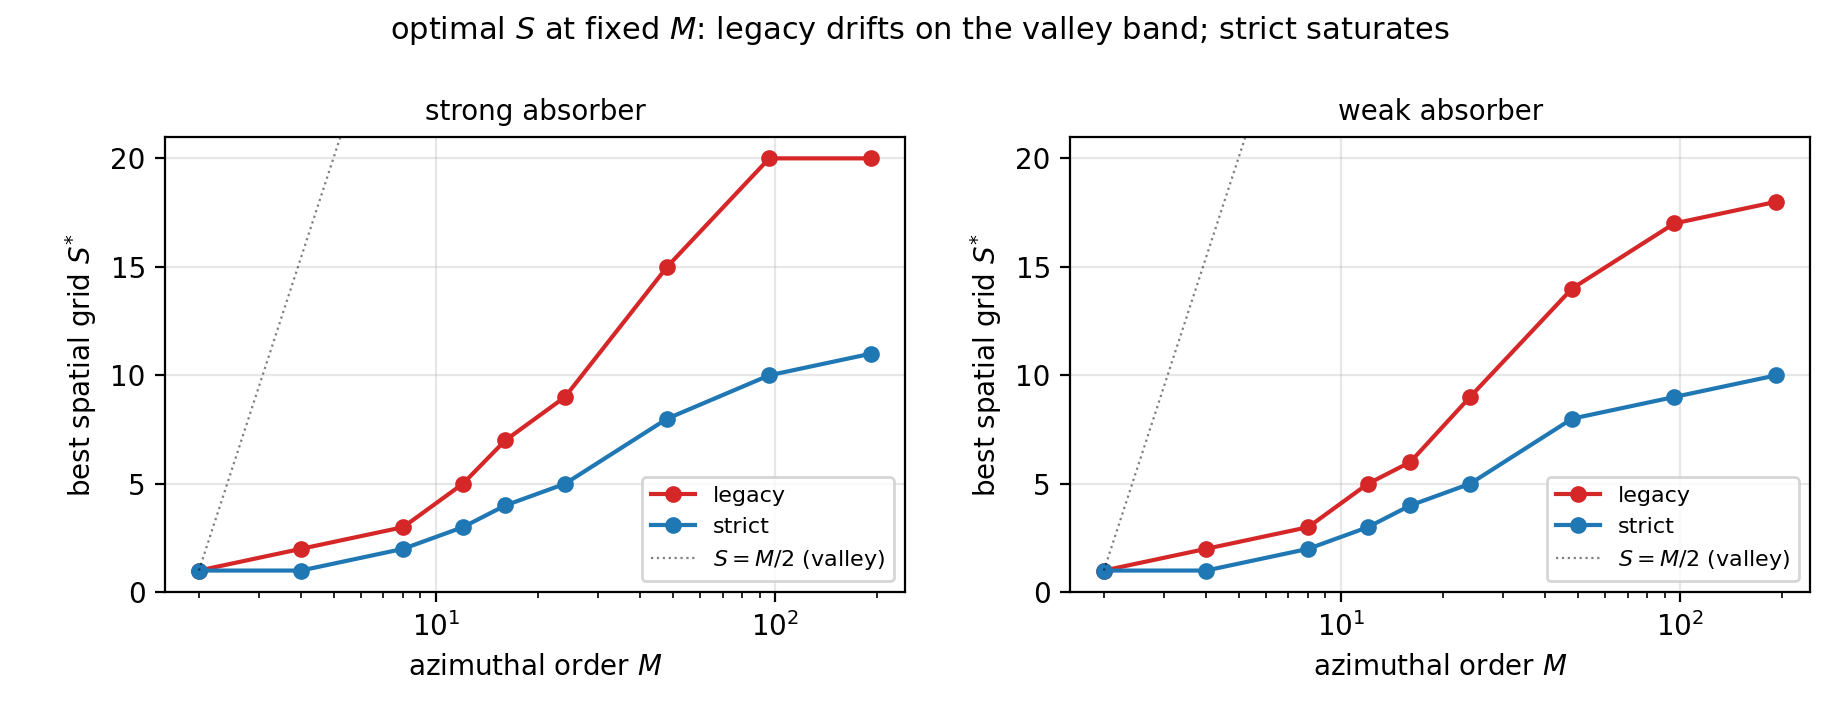
\includegraphics[width=\linewidth]{figures/fig_bestS.png}
\caption{Optimal spatial grid at fixed azimuthal order. Legacy $S^{*}$
tracks the cancellation band $S\approx M/2$ out of every finite grid;
strict $S^{*}$ saturates at the zero crossing of the spatial residual.}
\label{fig:bestS}
\end{figure}

\begin{figure}[t]
\centering
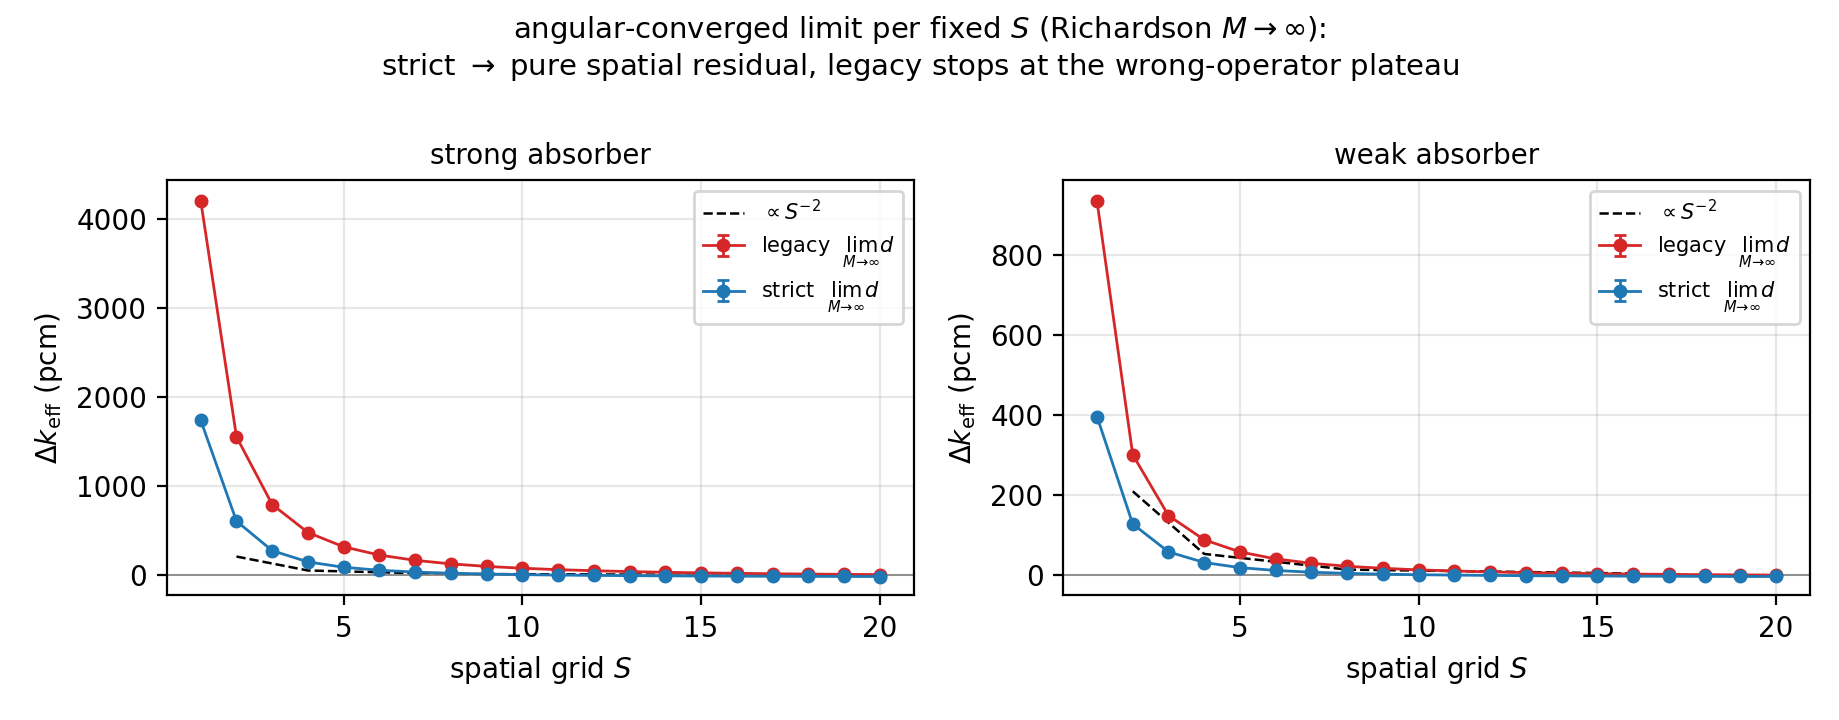
\includegraphics[width=\linewidth]{figures/fig_limits.png}
\caption{Richardson $M\to\infty$ limit of each fixed-$S$ row (error
bar: extrapolation self-disagreement). Strict limits form a single-signed
$\propto S^{-2}$ spatial-residual sequence; legacy limits plateau at the
body/face operator-error offset.}
\label{fig:limits}
\end{figure}

\end{document}
